\documentclass[notes,slidesec,a4]{seminar}
\usepackage[spanish]{babel}
\usepackage[utf8]{inputenc}
\usepackage{t-gsyc-6}
\usepackage{fancybox}
\usepackage{graphics}
\usepackage{moreverb}
\usepackage{alltt}
\usepackage{html}
\usepackage{hthtml}
\usepackage{amsmath}
\usepackage[normalsize]{subfigure}
\usepackage{url}
\usepackage{listings}
\usepackage{eurosym}

\title{\color{red}{BT-Studio: a ROS Behavior Tree webIDE}}
\author{Asociación de Robótica e Inteligencia Artificial JdeRobot}
\cop{JdeRobot}
\address{CIF G88145909}
\date{josemaria.plaza@gmail.com, oscar.robotics@tutanota.com, javizqh@gmail.com}

\begin{document}
\maketitle


\begin{hslide}
\slsubsect{Contents}
\begin{itemize}
\item Who we are
\item Introduction
\item BT-Studio tool
  \begin{itemize}
  \item Features
  \item Graphical User Interface
  \item Edit: Visual BT editor
  \item Edit: Action files
  \item Run Monitored execution
  \item Examples
  \end{itemize}
\item How is it done?
\item Conclusions
\end{itemize}
\end{hslide}

\begin{hslide}
\slsect{JdeRobot: who we are}

\begin{minipage}[t]{8.8cm}
  \begin{itemize}
\item International open source robotics organization, 2014-
\item \texttt{https://jderobot.github.com}
\item Projects
  \begin{itemize}
  \item Robotics education: RoboticsAcademy
  \item Robot programming tools: Unibotics, BT-Studio...
  \item AI driven robotics
  \end{itemize}
\item Activities: Google Summer of Code, internships...
\item Community: 20+
\end{itemize}
\end{minipage}
\begin{minipage}[t]{3cm}
 \begin{figure}
    %    \begin{center}    
      
\includegraphics[width=3cm]{logo-jderobot.png}
%    \end{center}
 \end{figure}
\end{minipage}
\end{hslide}

\begin{hslide}
  \vspace{-0.3cm}
  \slsect{Introduction}
  \vspace{-0.4cm}
%\begin{minipage}[t]{7cm}
\begin{itemize}
\item Reactive approach does not scale up to complex robotics applications 
\item ``Planned execution'': Finite State Machines, Behavior-Trees (BT)...
  %\item Uo to date with modern developer trends like the use of Behavior Trees in IA
  %\item Tries to improve on already established tools, for example: Groot and Groot2.
%\item Actions, nodes, decorators...
\item \textcolor{blue}{Simplify and speed up the development of BT robotics applications}
%\item Making Behavior-Trees more accesible: web browser
\item Maximize compatibility with state of the art technologies:\\
  \texttt{BehaviorTrees.CPP} (+groot2), \texttt{Py\_Trees}
  %\item Fast and streamlined development of fairly complex applications with the 3.8 version according to BehaviorTrees.CPP.
%\item Reuse of behavior trees and modification in a graphical interface.
\end{itemize}
%\end{minipage}
\begin{minipage}[t]{7cm}
  \vspace{-0.5cm}
  \begin{figure}
    %    \begin{center}    
      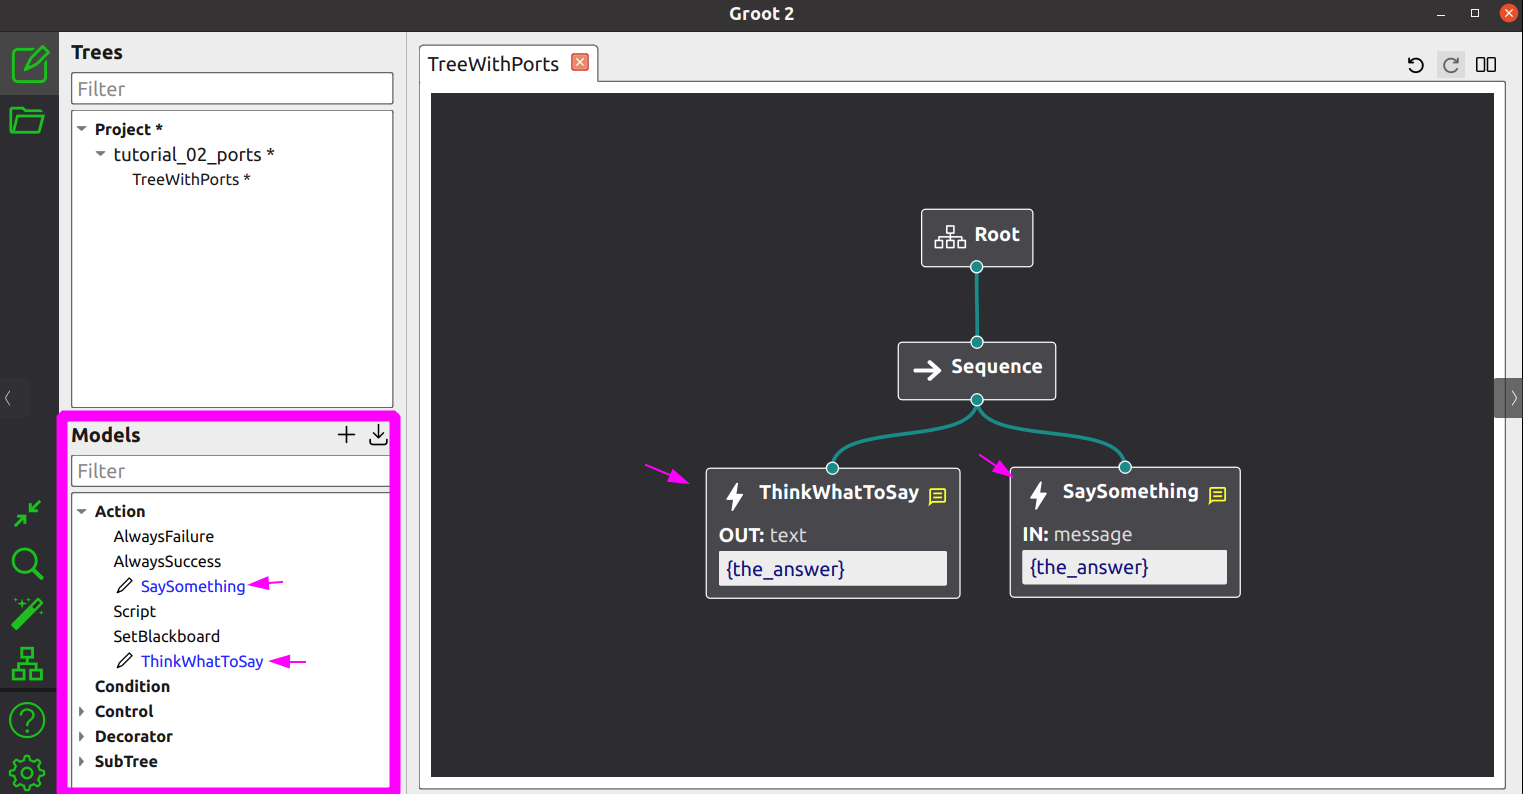
\includegraphics[width=6.5cm]{figs/groot2.png}
%    \end{center}
  \end{figure}
\end{minipage}
\begin{minipage}[t]{5cm}
%  \vspace{0.2cm}
  \begin{itemize}
  \item Actions
  \item Sequence, Fallbacks
  \item Decorators
  \end{itemize}
\end{minipage}
\end{hslide}

\begin{hslide}
\slsect{BT Studio tool}
\centerline{\textit{\textcolor{red}{Web based IDE: edit, run, debug robotics applications from the browser}}}
\vspace{0.2cm}
\slsubsect{Features}
\vspace{-0.2cm}
\begin{itemize}
\item Crossplatform (Linux, Windows, MacOS)
\item Python applications 
\item ROS2 Humble
\item Simulated (Gazebo, Webots...) and real robots 
\item Open-source: \texttt{https://github.com/JdeRobot/bt-studio}
%\item \texttt{https://jderobot.github.io/bt-studio/}
\item Each user has a set of \textcolor{blue}{robotics projects}, each project several files
\end{itemize}

\newpage
\slsubsect{User Interface}
\vspace{-0.3cm}
\begin{itemize}
\item Files (Application [actions, trees], Universes...)
\item \textit{Text editor} for Python Actions, \textit{Visual editor} for BT
\item Execution monitoring: \textit{VNC viewer}
%\item Program the actions while modifying the behaviour tree \normalsize
\end{itemize}
\begin{center}
  \begin{figure}
    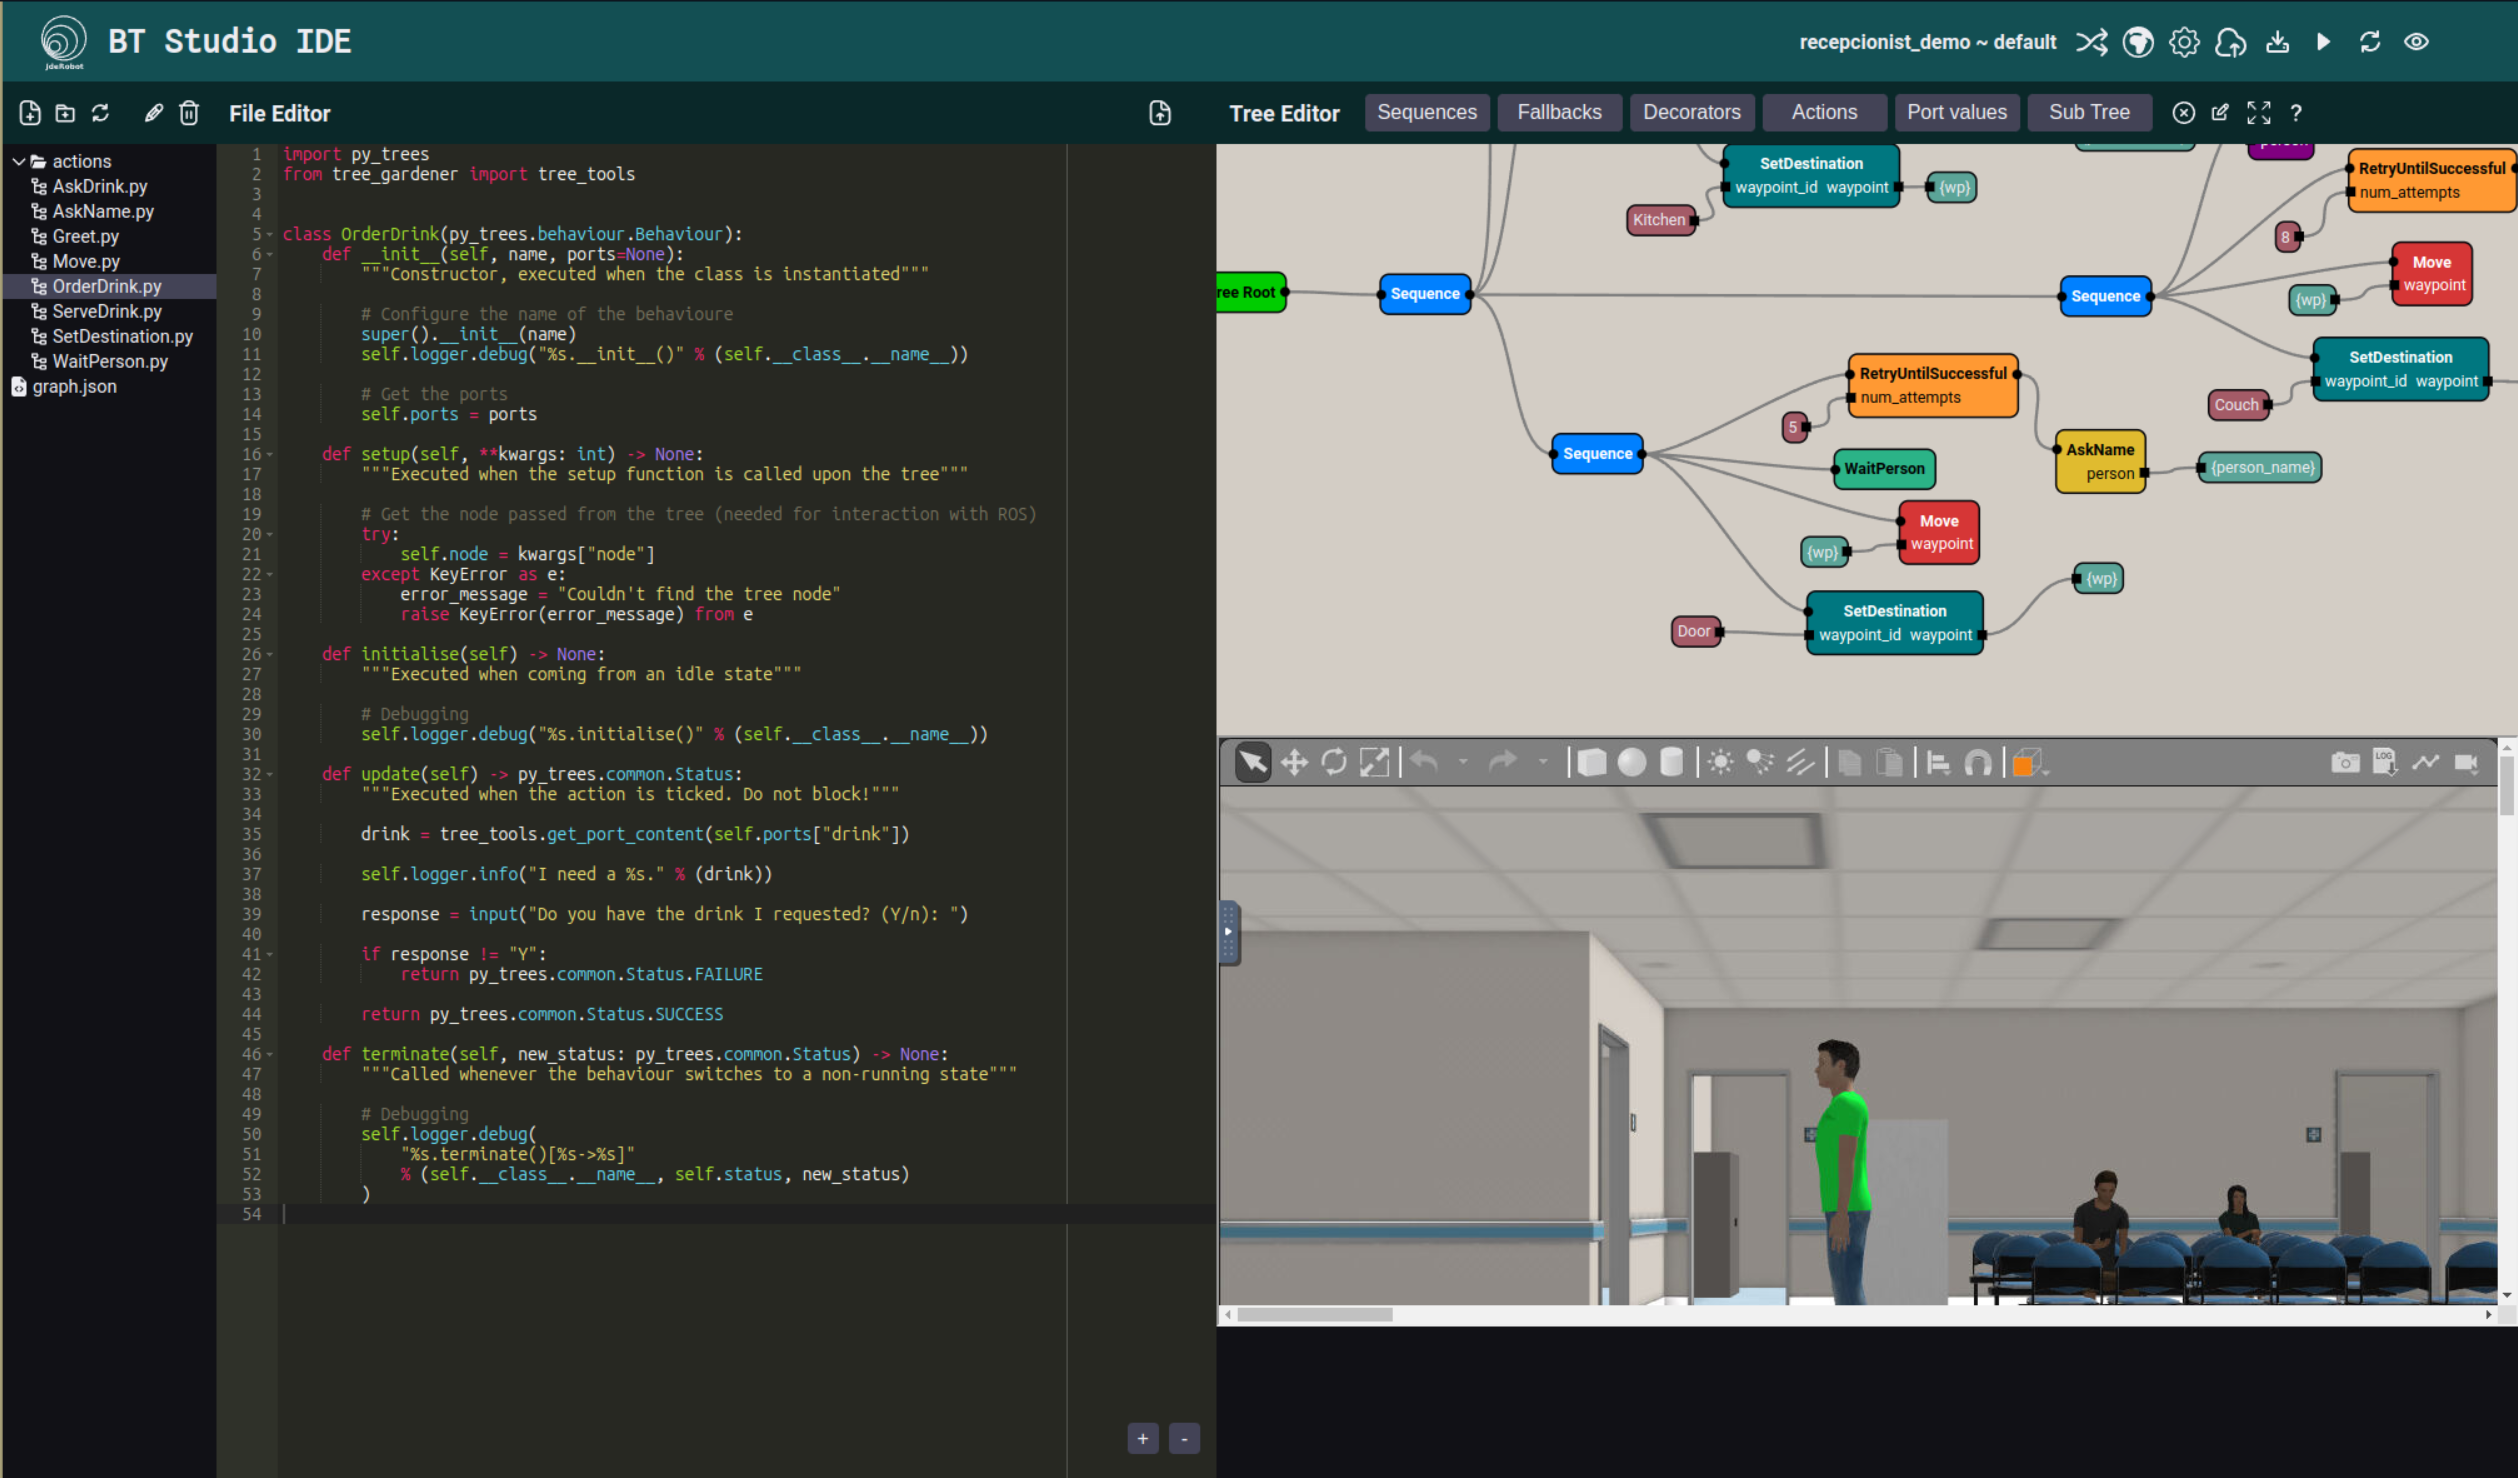
\includegraphics[width=8.5cm]{figs/BtStudio0.6-2.png}
     \end{figure}
\end{center}


%%   \newpage
%%   \slsubsect{Features}
%% \begin{itemize}
%% 	\item Manage multiple projects
%% 	\item Manage multiple universes
%% %	\item Programming in the \textcolor{blue}{Python} language
%% 	\item Edit the behavior tree actions in the diagram editor 
%% 	\item Define the behaviour tree structure using a graphical interface
%% %	\item Both on real robots and on simulated robots (Gazebo, Webots...)
%% 	\item Integrated Vnc visualizer for dockerized execution
%% \end{itemize}
  


\newpage
\slsubsect{Edit: Visual BehaviorTree editor}
\hspace{-0.5cm}
\begin{minipage}[t]{5.7cm}
  \vspace{0.5cm}
\begin{itemize}
\item Intuitive reactive \textcolor{blue}{REACT editor}
\item Customizable colors for each action
\item Configurable order:\\ bottom$\rightarrow$top, top$\rightarrow$bottom, ...
\item Actions
\item Sequence, Fallbacks
\item Decorators
\end{itemize}
\end{minipage}
\begin{minipage}[t]{6cm}
	\begin{center}
	\begin{figure}
		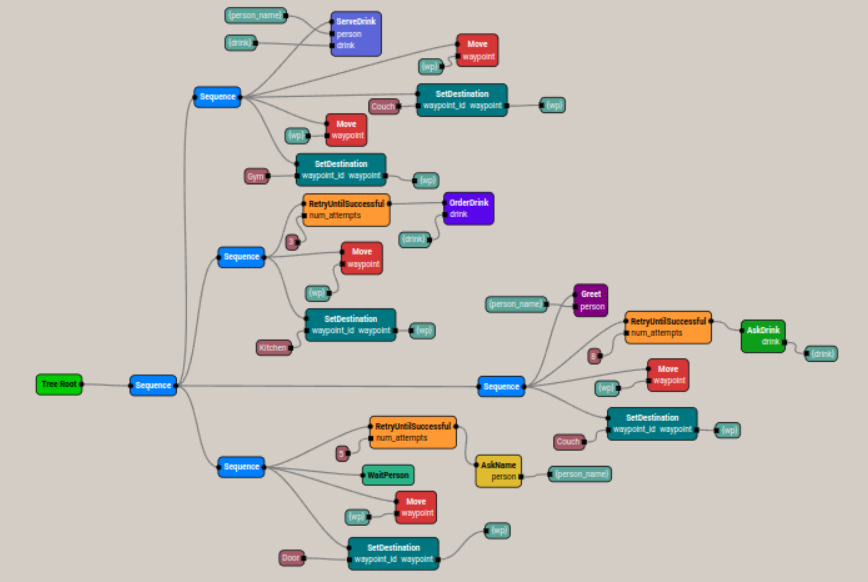
\includegraphics[width=5.7cm]{figs/BtStudio0.6-4.png}
	\end{figure}
        \end{center}
\end{minipage}
%\end{minipage}


\newpage
\slsubsect{Edit: Action files}
\vspace{-0.6cm}
  \begin{minipage}[t]{5.5cm}
	\begin{center}
	\begin{figure}
		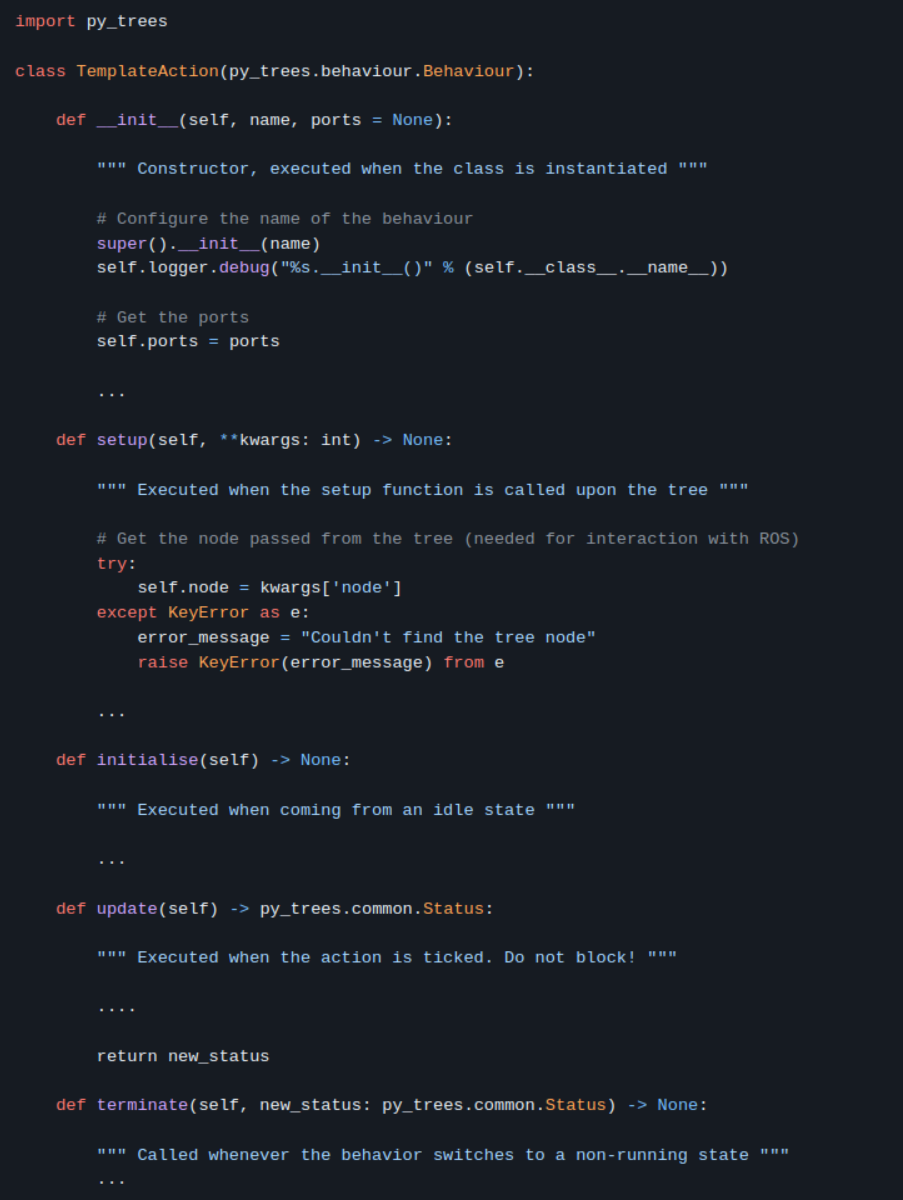
\includegraphics[width=4.9cm]{figs/screenshot4.png}
	\end{figure}
        \end{center}
  \end{minipage}
  \begin{minipage}[t]{6cm}
    \vspace{0.3cm}
    \begin{itemize}
    \item Same structure as py\_trees actions
    \item Setup
    \item Initialise
    \item Update
    \item Terminate
    \end{itemize}
\begin{center}
	\begin{figure}
		\includegraphics[width=1.8cm]{figs/BTStudio0.6-5.png}
	\end{figure}
        \end{center}
   \end{minipage}

\newpage
 \slsubsect{Run: Monitored execution}
 \begin{itemize}
 \item (1) \textcolor{blue}{Dockerized execution} (\textit{Robotics Backend})
 \small
   \begin{itemize}
   \item All dependencies, assets, etc... are already pre-installed     
   \end{itemize}
   \normalsize
 \item (2) Local execution creating a ROS2 package
   \small
   \begin{itemize}
   \item ROS2 Humble is required installed locally
   \item A test enviroment is provided with Webots simulator and a tree execution visualizer as thirdparty repos
%   \item Run the app using an specific executor     
   \end{itemize}
   \normalsize
 \vspace{1cm}
 \item Control the flow of execution: Run, Pause and Restart
 \item \textcolor{blue}{Simple selection of Universes}\\ (simulated worlds, robot models, launchers...)
 %	\item Using the Robotics Backend docker for easy development and ready to use templates.
 \end{itemize}
 
\newpage
\slsubsect{Examples}
\hspace{-1.cm}
\begin{minipage}[t]{7cm}
  %  \vspace{0.5cm}
  \begin{figure}
    %  \hspace{1.5cm}
    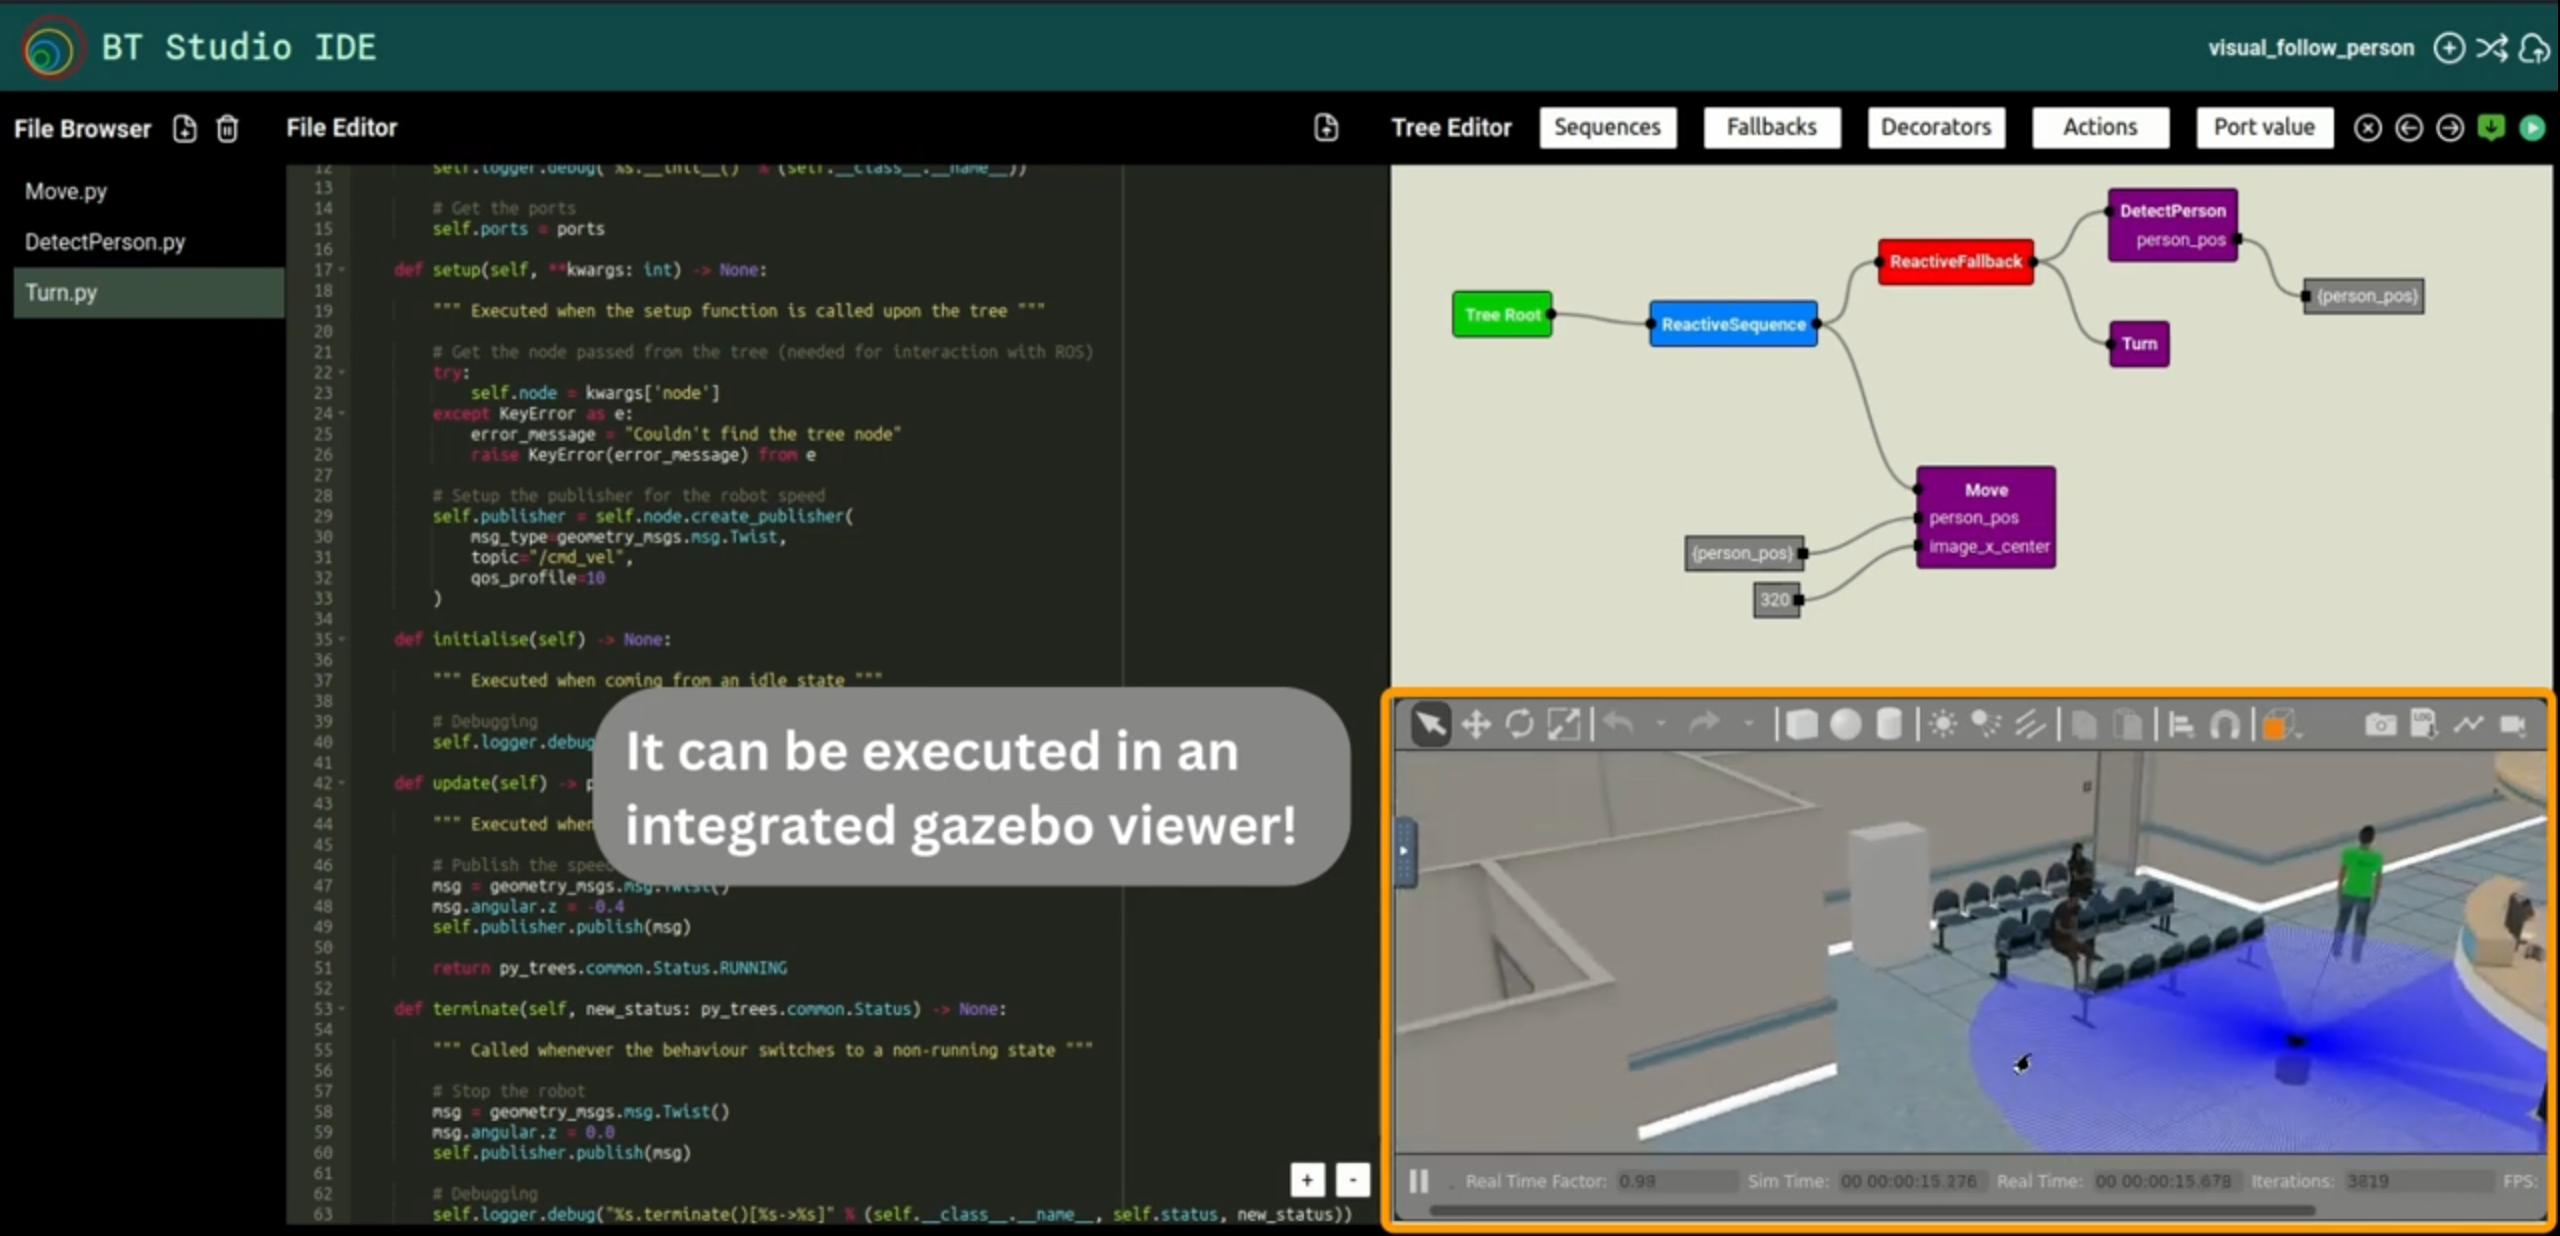
\includegraphics[width=7cm]{figs/demo-followperson.png}
  \end{figure}
  \begin{itemize}
           \item \href{https://youtu.be/a4c-nRevF_c}{Follow Person application}
  \end{itemize}
\end{minipage}
  \begin{minipage}[t]{6cm}
  \begin{figure}
    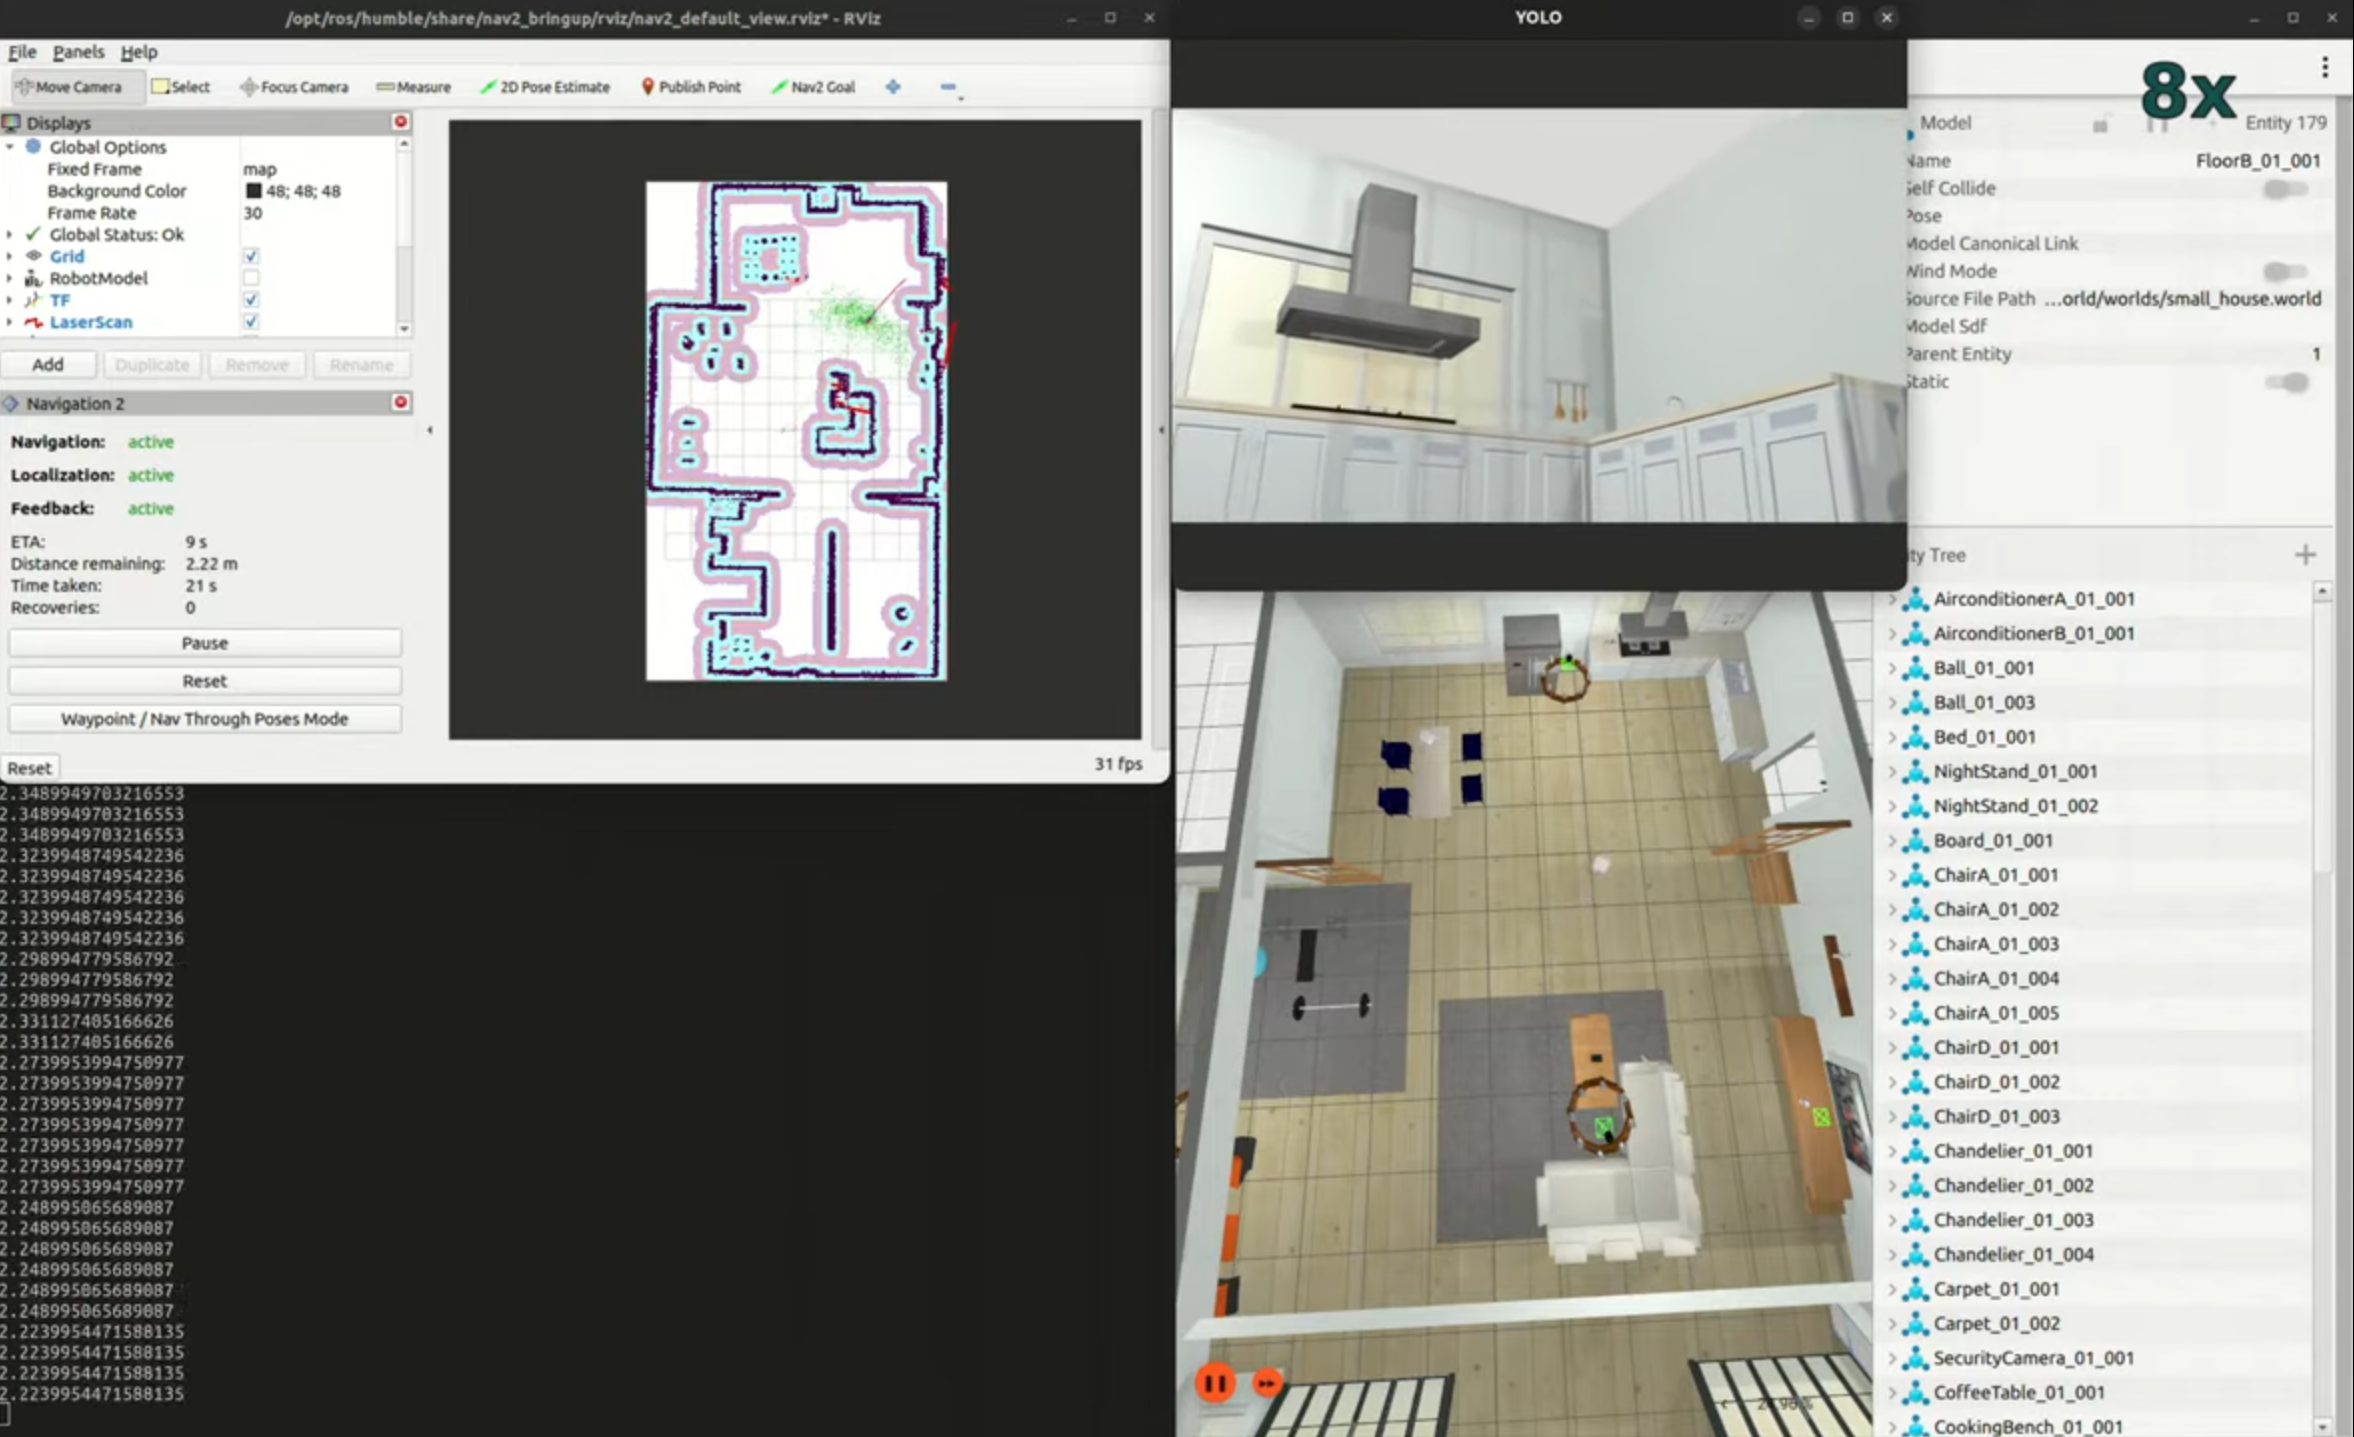
\includegraphics[width=6cm]{figs/demo-robocup2022.png}    
  \end{figure}
  \begin{itemize}
  \item \href{https://youtu.be/yZZWjFbdt_4}{RoboCup2022 recepcionist}        
  \end{itemize}
\end{minipage}
\end{hslide}

\begin{hslide}
\slsect{How is it done?}
\begin{minipage}[t]{7cm}
    \begin{itemize}
    \item Web tecnologies
      \begin{itemize}
      \item backend: Django
      \item frontend: React, HTML5, CSS
        %websockets
      \end{itemize}
    \item Robotics tecnologies
      \begin{itemize}
      \item ROS2
      \item Py\_trees
      \item Gazebo, Webots simulators
      \end{itemize}
    \item DevOps tecnologies
      \begin{itemize}
      \item Docker
      \item VNC
      \end{itemize}
    \end{itemize}
\end{minipage}
\begin{minipage}[t]{5cm}
  \begin{figure}
    \centerline{
\includegraphics[width=4cm]{figs/html5.png}}
    
\includegraphics[width=1.5cm]{figs/Django-Logo.png}
    
\includegraphics[width=2cm]{figs/react-logo.png}
    
\includegraphics[width=1.6cm]{figs/docker-logo.png}\\
    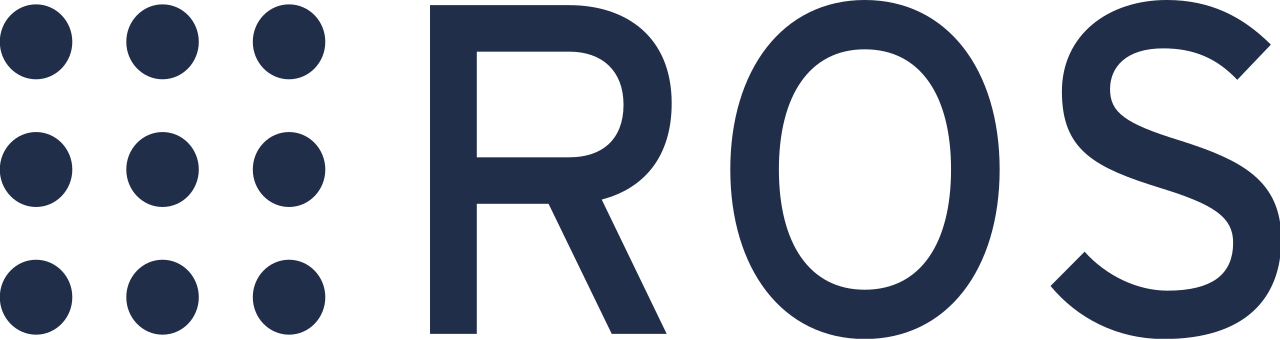
\includegraphics[width=1.5cm]{figs/Ros-logo.png}
  \end{figure}
\end{minipage}


\newpage
\slsubsect{Internal files}
  \begin{minipage}[t]{7cm}
	\vspace{1cm}
  	\begin{itemize}
	  	\item \texttt{app\_tree.xml}: BT and source code
		\item \texttt{execute.py}:\\launcher for the application
		\item \texttt{execute\_docker.py}:\\ launcher for dockerized execution
		\item Auxiliary files as a basic ROS2 package
	\end{itemize}
  \end{minipage}
  \begin{minipage}[t]{5cm}
  	\begin{figure}
  		\centerline{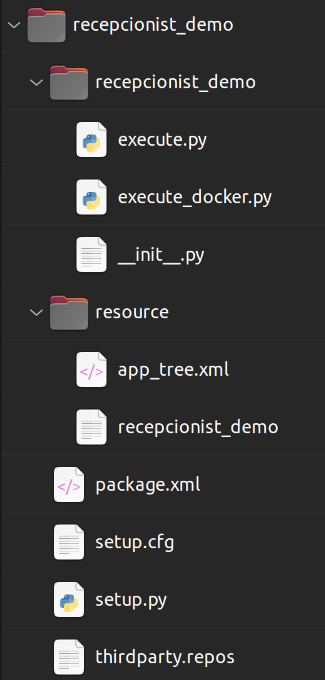
\includegraphics[width=2.8cm]{figs/package-struct.png}}
  	\end{figure}
  \end{minipage}


\newpage
 \slsubsect{Translation process}
 \begin{itemize}
 \item \textit{From the user Python code for the Actions and the visual BT diagram to executable Python files}
 \item It is done in the backend
 \item Both are combined into a \textcolor{blue}{single XML file} with 2 sections:
   \begin{itemize}
 \item BehaviorTree section with the same structure as Groot2 BT
 \item Code section is used instead of external files
   \end{itemize}
 \end{itemize}  
\end{hslide}


\begin{hslide}
  \slsect{Conclusions}
\begin{itemize}
\item Context: Flowstate (Intrinsic), MoveIt Pro (Picknik), TheConstruct...
\item Faster and simpler development of Behavior-Tree robotics applications
\item Edit, run and debug BT robotics applications \textcolor{blue}{from the web browser}
  \end{itemize}
  \vspace{1cm}  
  \begin{itemize}
  \item Integration in Unibotics, our robot programming website
  \item Library of reusable subtrees (Google Summer of Code 2024)
  \item Library of universes
%  \item Release 1.0
  \end{itemize}
\end{hslide}

\end{document}

